\documentclass[12pt]{article}

\usepackage{multicol}
\usepackage[margin=0.75in]{geometry}
\usepackage{titlesec}
\usepackage{amsmath}
\usepackage[
backend=biber,
style=ieee,
sorting=ynt
]{biblatex}
\usepackage{fancyhdr}
\usepackage{enumitem}
\usepackage{graphicx}
\usepackage{float}

% \pagestyle{fancy}
%\fancyhf{}

\title{ECE419 M1 Report}
\date{28 January 2018}
\author{Thomas Kingsford\\Marcel Mongeon\\Zhihao Sheng}

%\titleformat{\section}{\normalfont\scshape}{\thesection}{1em}{}
%\titlespacing*{\section}{0pt}{10pt}{0pt}

%\setlength{\parindent}{0pt}
%\setlength{\parskip}{0cm}
%\renewcommand{\baselinestretch}{0.5}
%\setlist{noitemsep} % {nosep, noitemsep}

\begin{document}
\begin{multicols}{2}
\maketitle

\section{Design and Decisions}

\paragraph{Architecture} Refer to Figure \ref{arch} in the Appendices for an architecture diagram.

\paragraph{KVClient} 

\paragraph{KVStore}

\paragraph{KVServer}

\paragraph{CommMod}

\paragraph{TLVMessage} The TLVMessage is an implementation of the KVMessage interface. it implements a modification of tag-length-value encoding. It (un)marshals a KV message as a sequence of bytes in which:

\begin{enumerate}
\item The first byte is the ordinal value of the StatusType enum, referred to as a 'tag'.
\item The second byte is the length of the key $L_K \in [0, 255]$. This protocol imposes an upper limit on key size of 255 bytes.
\item For messages containing a value (the existence of a value is fully determined by the tag), the third byte is the length of the value $L_V \in [0, 255]$. This protocol imposes an upper limit on key size of 255 bytes. This could be trivially extended - for instance, the use of four bytes would give a maximum length of $2^32-1\approx 1 \text{ billion bytes}$
\item The following $L_K$ bytes are the key.
\item If there is a value, the following $L_V$ bytes are the value.
\end{enumerate}

\paragraph{LRUCache}

\paragraph{LFUCache}

\paragraph{FIFOCache}

\paragraph{LockManager}

\paragraph{FilePerKeyKVDB}


\section{Performance Evaluation}


\section{Test Cases}

\subsection{CacheTests}

\subsection{CommModTests}

\subsection{ConnectionTest}

\subsection{InteractionTest}

\subsection{KVDBTests}

\subsection{LockManagerTest}

\subsection{SocketTest}

\subsection{StoreServerTests}

\subsection{TLVMessageTest}

\end{multicols}

\newpage

\section{Appendices}

\begin{figure}[H]
\centering
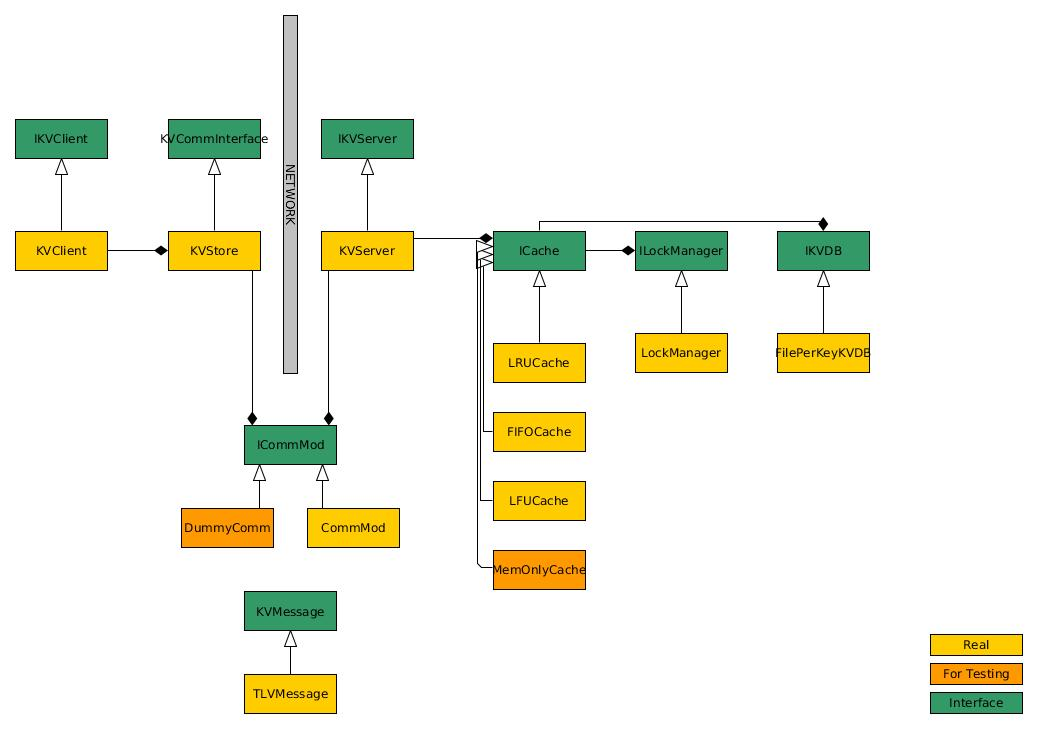
\includegraphics[scale=0.50]{architecture}
\caption{Architecture Diagram}
\label{arch}
\end{figure}
\end{document}

